\documentclass[12 pt]{extarticle}

	\usepackage[frenchb]{babel}
	\usepackage[utf8]{inputenc}  
	\usepackage[T1]{fontenc}
	\usepackage{amssymb}
	\usepackage[mathscr]{euscript}
	\usepackage{stmaryrd}
	\usepackage{amsmath}
	\usepackage{tikz}
	\usepackage[all,cmtip]{xy}
	\usepackage{amsthm}
	\usepackage{varioref}
	\usepackage{geometry}
	\geometry{a4paper}
	\usepackage{lmodern}
	\usepackage{hyperref}
	\usepackage{array}
	 \usepackage{fancyhdr}
\renewcommand{\theenumi}{\alph{enumi})}
	\pagestyle{fancy}
	\theoremstyle{plain}
	\fancyfoot[C]{} 
	\fancyhead[L]{Contrôle}
	\fancyhead[R]{2 octobre 2023}\geometry{
 a4paper,
 total={170mm,257mm},
 left=20mm,
 top=20mm,
 }
	
	
	\title{Contrôle Chapitre 1}
	\date{}
	\begin{document}

\begin{center}{\Large Chapitre 1 - Rappels de  numération}\\ 
 \end{center}
 
 \subsection*{Exercice 1}
On considère le nombre $1264,875$. Recopier et compléter les affirmations suivantes. 
 \begin{enumerate}
 \item Le chiffre des milliers est \ldots.
 \item Le chiffre des centièmes est \ldots. 
 \item Le chifre des \ldots est la somme du chiffre des \ldots et du chiffre des \ldots. 
 \item La partie entière est \ldots, et la partie décimale est \ldots. 
 \item Le produit des chiffres de la partie entière est \ldots. 
 \end{enumerate}

\subsection*{Exercice 2}

Compléter le tableau suivant. 

\renewcommand{\arraystretch}{2}
\begin{tabular}[height = 15 pt]{|l|l|l|l|}
\hline 
nombre décimal & fraction décimale  & somme d'un entier et d'une fraction décimale $<1$\\ \hline
$1,23$ &  &  \\
\hline 
 &  $\displaystyle\frac{76402}{100}$ &  \\
\hline 
 &  & $\displaystyle123 + \frac{12}{100}$   \\
\hline 
 &  $\displaystyle\frac{764}{10\ 000}$ &  \\
\hline 
 &  & $\displaystyle653 + \frac{76}{1000}$   \\
\hline
\end{tabular}

\subsection*{Exercice 3}

Calculer : \begin{enumerate}
\item $120 \div 100$
\item $0,123 \times 100$
\item $12, 54 \div 1000$
\item $ 54,12 \times 1000$
\end{enumerate}

\subsection*{Exercice 4}
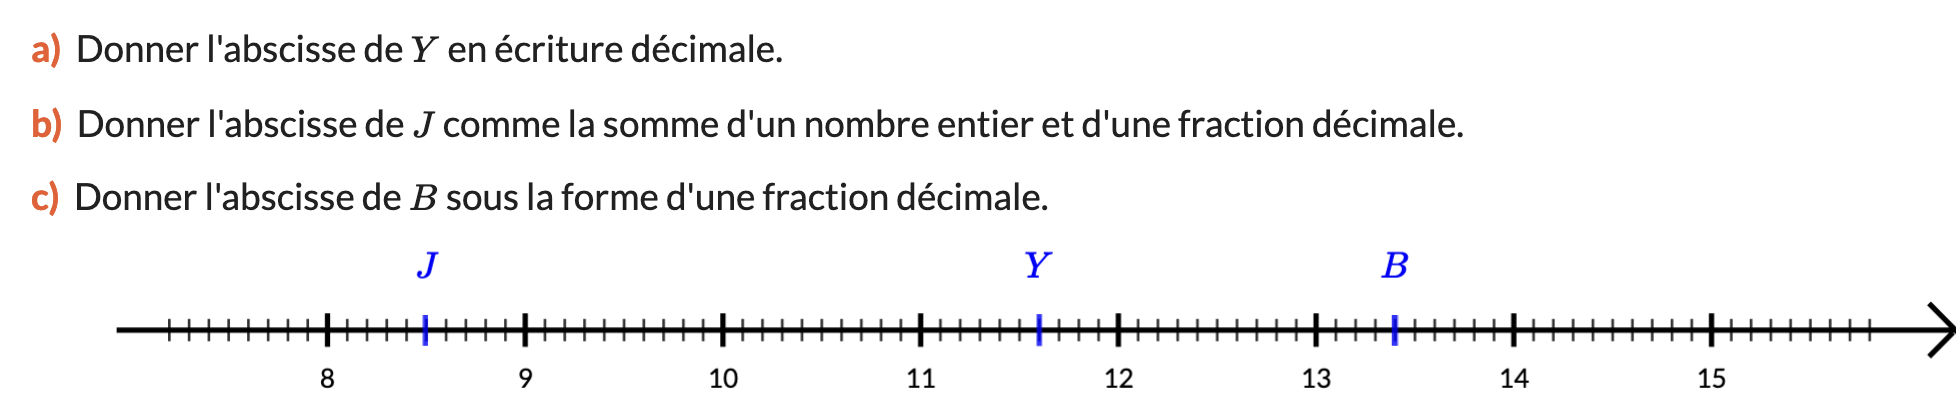
\includegraphics[scale=0.5]{Exo4a}


\newpage


\begin{center}{\Large Chapitre 1 - Rappels de  numération}\\ 
 \end{center}
 
 \subsection*{Exercice 1}
On considère le nombre $2364,405$. Recopier et compléter les affirmations suivantes. 
 \begin{enumerate}
 \item Le chiffre des milliers est \ldots.
 \item Le chiffre des centièmes est \ldots. 
 \item Le chifre des \ldots est la somme du chiffre des \ldots et du chiffre des \ldots. 
 \item La partie entière est \ldots, et la partie décimale est \ldots. 
 \item Le produit des chiffres de la partie entière est \ldots. 
 \end{enumerate}

\subsection*{Exercice 2}

Compléter le tableau suivant. 

\renewcommand{\arraystretch}{2}
\begin{tabular}[height = 15 pt]{|l|l|l|l|}
\hline 
nombre décimal & fraction décimale  & somme d'un entier et d'une fraction décimale $<1$\\ \hline
$1,23$ &  &  \\
\hline 
 &  $\displaystyle\frac{76052}{100}$ &  \\
\hline 
 &  & $\displaystyle129 + \frac{12}{100}$   \\
\hline 
 &  $\displaystyle\frac{974}{10\ 000}$ &  \\
\hline 
 &  & $\displaystyle643 + \frac{76}{1000}$   \\
\hline
\end{tabular}

\subsection*{Exercice 3}

Calculer : \begin{enumerate}
\item $0,653 \times 100$
\item $650 \div 100$
\item $12, 45 \div 1000$
\item $ 34,12 \times 1000$
\end{enumerate}

\subsection*{Exercice 4}
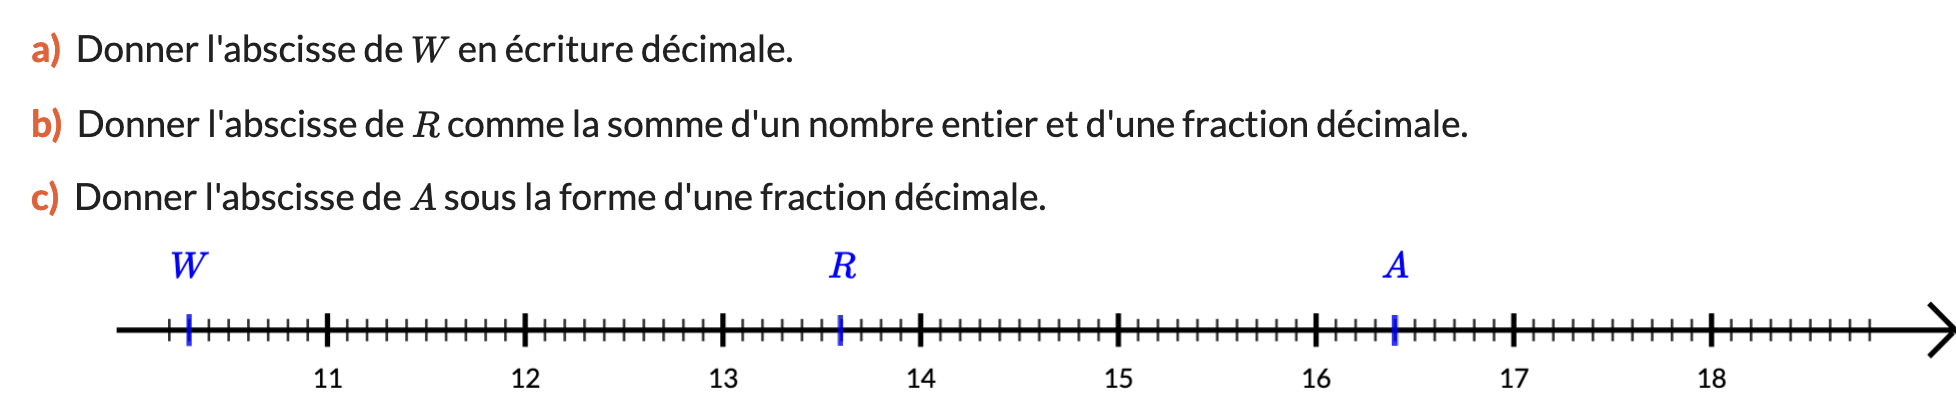
\includegraphics[scale=0.5]{Exo4a'}
 	\end{document}
